\documentclass[letterpaper,11pt]{article}

\author{Jacob Thomas Errington}
\title{Assignment \#2\\Formal verification -- COMP 525}
\date{7 February 2017}

\usepackage[margin=2.0cm]{geometry}
\usepackage{amsmath,amsthm,amssymb}

\usepackage{tikz}
\usetikzlibrary{graphs, arrows}

\newtheorem{prop}{Proposition}
\newtheorem{claim}{Claim}

\renewcommand{\thesection}{Q\arabic{section}}

\newcommand{\Z}{\mathbb{Z}}
\newcommand{\N}{\mathbb{N}}
\newcommand{\union}{\cup}
\newcommand{\intersn}{\cap}
\newcommand{\up}{\uparrow}
\DeclareMathOperator{\Pref}{Pref}
\DeclareMathOperator{\FairPaths}{FairPaths}
\DeclareMathOperator{\MBP}{MinBadPrefs}
\DeclareMathOperator{\BP}{BadPrefs}
\let\L\undefined
\DeclareMathOperator{\L}{\mathcal{L}}

\newcommand{\state}[2]{$\left\langle#1,#2\right\rangle$}

\newcommand{\enumalpha}{\renewcommand\labelenumi{(\alph{enumi})}}

\begin{document}

\maketitle

\section{(\# 3.5) Formalizing linear-time properties}

We consider the set of atomic propositions $AP = \{x = 0, x > 1\}$ and a
nonterminating sequential program $P$ that manipulates $x$. We formalize the
following informal linear-time properties. Let $\Sigma = 2^{AP}$.

\begin{enumerate}
        \enumalpha \setcounter{enumi}{4}
    \item ``$x$ exceeds one only finitely many times''

        This is formalized by the $\omega$-regular expression
        $P = \Sigma^* (\Sigma \setminus \{ \{x>1\} \})$.
        (We do not exclude $\{x>1, x=0\}$ since it is impossible anyway.)

        This property is \emph{not} a satefy property. To show this we find a
        counterexample. Consider the string $\sigma = \{x > 1\}^\omega$. Take
        an arbitrary finite prefix $\hat \sigma < \sigma$. It consists of some
        finite number of $\{x > 1\}$. Notice that
        $\bar \sigma = \{x > 1\}^n \emptyset^\omega \in \hat \sigma \up$ and
        $\bar \sigma \in P$. Hence the set of extensions of $\hat \sigma$ has
        nonempty intersection with $P$. This establishes that $P$ is not a
        safety property.

    \item ``$x$ exceeds one infinitely often''

        We use the $\omega$-regular expression
        $\Sigma^* (\Sigma^* \{x>1\})^\omega$.

        This also not a safety property by a similar argument involving a
        string consisting a finite number of $\{x > 1\}$. Any finite prefix of
        this string can be extended with $\{x > 1\}^\omega$ giving a string in
        $P$.

    \item ``the value of $x$ alternates between zero and two''

        There is no way to determine using only the given atomic propositions
        that $x$ has the value two. We make the following assumption:
        $x \in \Z_3$. Hence $x > 1 \iff x = 2$.

        Then, we use the $\omega$-regular expression
        $P = (\{x=0\}\{x>1\})^\omega + (\{x>1\}\{x=0\})^\omega$.

        This is a safety property. Take arbitrary $\sigma \notin P$. By
        definition, there must be some point -- say, at the
        $n$\textsuperscript{th} position -- in the string where $\{x = 0\}$ is
        not followed by $\{x > 1\}$ (or vice versa). Any extension of the
        prefix going up to and including this first repetition will clearly
        still exhibit the problematic repetition.

    \item ``true''

        To construct a family of sets of atomic propositions that is always
        satisfied, it suffices to take the whole set, and subtract the
        impossible case $\{x=0, x>1\}$. Let
        $Q = \Sigma \setminus \{x = 0, x > 1\}$

        This gives the $\omega$-regular expression
        $P = Q^\omega$.

        This is a safety property. As soon as a point in the string is reached
        such that the impossible case $\{x = 0, x > 1\}$, any extension of this
        string cannot ``go back in time'' to fix the fact that this bad thing
        happened.
\end{enumerate}

\section{(\# 3.6) Classifying linear-time properties}

\begin{enumerate}
        \enumalpha
    \item ``$A$ should never occur''

        This can be formalized by the $\omega$-regular expression
        \begin{equation*}
            P = (\Sigma \setminus \{ \{A\}, \{A, B\} \})^\omega
        \end{equation*}

        This is an invariant, since there exists a formula $\phi = \neg A$ such
        that
        \begin{equation*}
            P = \left\{
                S_0 S_1 S_2 \ldots \in \Sigma^\omega
                | \forall j \geq 0 : A_j \models \phi
            \right\}
        \end{equation*}

    \item ``$A$ should occur exactly once''

        Let $Q = \Sigma \setminus \{ \{A\}, \{A, B\} \}$. Then, this property
        can be formalized by the $\omega$-regular expression
        \begin{equation*}
            P = Q^* \{A\} Q^\omega
        \end{equation*}

        This is not an invariant, because intuitively there's nothing we can
        say about the states individually that lets us know whether the
        property is satisfied or not. This is not a safety property either.
        Suppose we have an arbitrary run $\sigma \notin P$. Notice that the
        string $\{B\}^\omega$ is a possible choice for $\sigma$. However, any
        finite prefix of this string has as a possible extension the string
        containing exactly one ``letter'' that is a set containing $A$. This is
        not a liveness property either. Suppose we have an arbitrary
        $\hat \sigma \in \Sigma^*$. A possible choice for this $\hat \sigma$
        may have more than one letter containing $A$. Hence it is not the case
        that an arbitrary finite word can be extended to an infinite run
        satisfying the property.

    \item ``$A$ and $B$ alternate infinitely often''

        For any index $i$ at which $A$ is true, there exists an index
        $i^\prime \geq i$ such that $B$ is true, and vice versa.
        Let $\bar A = \{ \{A\}, \{A, B\} \}$
        and $\bar B = \{ \{B\}, \{A, B\} \}$.
        Then, we formalize the property with the $\omega$-regular expression
        \begin{equation*}
            P = \Sigma^* (\bar A \Sigma^* \bar B \Sigma^*)^\omega
        \end{equation*}

        This is a liveness property.
        Take an arbitrary $\hat \sigma \in \Sigma^*$.
        Then it can clearly be extended to a $\sigma \in P$.

    \item ``$A$ should eventually be followed by $B$''

        We understand this as a somewhat weaker version of the previous
        property. We adopt the notation introduced in the previous exercise,
        and additionally
        let $\hat A = \{ \emptyset, \{A\} \}$
        and $\hat B = \{ \emptyset, \{B\} \}$.
        We formalize this with the
        $\omega$-regular expression
        \begin{equation}
            \label{eq:trickysafeprop}
            P
            = (\hat B)^\omega
            + \Sigma^* (\bar A (\Sigma^* \{A, B\})^* \Sigma^* \{B\})^\omega
        \end{equation}

        This expression encodes the notion that if a letter involving $A$ is
        encountered, then at some point later in the string, a letter involving
        $B$ is found. This is tricky because the letter $\{A, B\}$ can serve
        both to terminate a forwards search for a $B$ and to``kick off''
        another search for $B$.

        This property is not a safety property. To see this, consider the
        string $\sigma = \{A\}^\omega$. Clearly this string does not satisfy
        the property. Consider an arbitrary finite prefix
        $\hat \sigma < \sigma$. By appending an infinite string of $\{B\}$ to
        this prefix, we obtain a string satisfying $P$, which contradicts the
        definition of a safety property.

        This property is however a liveness property. Given an arbitrary finite
        string $\hat \sigma \in \Sigma^*$, we can complete it to a string
        satisfying $P$ by following the second branch of the alternation in
        \eqref{eq:trickysafeprop}.
\end{enumerate}

\section{(\# 3.11) Closure properties of liveness and safety properties}

\begin{prop}
    Let $P$ and $P^\prime$ be liveness properties over $AP$. Then,
    \begin{enumerate}
        \item $P \union P^\prime$ is a liveness property.
        \item $P \intersn P^\prime$ is not, in general, a liveness property.
    \end{enumerate}
\end{prop}

\begin{proof}
    We show each statement separately.

    \begin{enumerate}
        \item
            Take arbitrary $\hat \sigma \in \Sigma^*$. Since $P$ is a liveness
            property, then $\hat \sigma \up \intersn P \neq \emptyset$.
            Likewise, $\hat \sigma \up \intersn P^\prime \neq \emptyset$.
            Observe
            \begin{align*}
                \hat \sigma \up \intersn (P \union P^\prime)
                = (\hat \sigma \up \intersn P)
                \union (\hat \sigma \up \intersn P^\prime)
                \neq \emptyset
            \end{align*}
            Hence, an arbitrary finite word can be extended into a run that
            satisfies $P$ or $P^\prime$, so
            $\hat \sigma \in \Pref(P \union P^\prime)$ which establishes that
            $\Pref(P \union P^\prime) = \Sigma^*$ and that $P \union P^\prime$
            is a liveness property.

        \item
            Consider that
            $P = \Sigma^* \{B\}^\omega$ and
            $P^\prime = \Sigma^* \{A\}^\omega$ are liveness properties.
            Notice that $P \intersn P^\prime = \emptyset$,
            so $\Pref(P \intersn P^\prime) = \emptyset \neq \Sigma^*$, which
            establishes that $P \intersn P^\prime$ is not a liveness property.
    \end{enumerate}
\end{proof}

\begin{prop}
    Let $P$ and $P^\prime$ be safety properties over $AP$. Then,
    \begin{enumerate}
        \item $P \union P^\prime$ is a safety property.
        \item $P \intersn P^\prime$ is a safety property.
    \end{enumerate}
\end{prop}

\begin{proof}
    We show each statement separately.

    \begin{enumerate}
        \item
            Take arbitrary $\sigma \notin P \union P^\prime$. Hence,
            $\sigma \notin P$ and $\sigma \notin P^\prime$. Since these are
            safety properties, there exist $\hat \sigma_P < \sigma$ and
            $\hat \sigma_{P^\prime} < \sigma$. Let $\hat \sigma$ be a
            string among these two with maximal length, and note that it is a
            bad prefix for both $P$ and $P^\prime$.
            \begin{equation*}
                \hat \sigma \up \intersn (P \union P^\prime)
                = \hat \sigma \up \intersn P
                \union \hat \sigma \up \intersn P^\prime
                = \emptyset \union \emptyset
                = \emptyset
            \end{equation*}

            This establishes that for any trace violating $P \union P^\prime$,
            we can find a bad prefix, so $P \union P^\prime$ is a safety
            property.

        \item
            Take arbitrary $\sigma \notin P \intersn P^\prime$.
            Hence, $\sigma \notin P$ or $\sigma \notin P^\prime$.
            \begin{description}
                \item[Case] $\sigma \notin P$.

                    Since $P$ is a safety property, we obtain
                    $\hat \sigma < \sigma$ such that
                    $\hat \sigma \up \intersn P = \emptyset$.
                    Hence,
                    \begin{equation*}
                        \hat \sigma \up \intersn (P \intersn P^\prime)
                        = (\hat \sigma \up \intersn P) \intersn P^\prime
                        = \emptyset \intersn P^\prime
                        = \emptyset
                    \end{equation*}

                \item[Case] $\sigma \notin P^\prime$. The same argument
                    applies, only with our attention focussed on $P^\prime$
                    instead.
            \end{description}

            This establishes that for any trace violating
            $P \intersn P^\prime$, we can find a bad prefix, so
            $P \intersn P^\prime$ is a safety property.
    \end{enumerate}
\end{proof}

\section{(\#3.17) Satisfaction under fairness assumptions}

\begin{prop}
    The trasition system $TS$ does not satisfy the (informally stated) property
    ``eventually $a$'' under the fairness assumptions $\mathcal{F}$.
\end{prop}

\begin{proof}
    Consider the execution
    \begin{equation*}
        \rho = (s_3 \beta s_4 \alpha s_5 \alpha s_4 \beta s_6 \beta)^\omega
    \end{equation*}
    This execution satisfies the required fairness conditions, namely if
    the action $X$ is enabled infinitely often, then that action is taken
    infinitely often, where $X = \alpha, \beta$. This means that $\rho$ is a
    fair path. However, this run never reaches the state $s_1$ in which the
    desired atomic proposition $a$ is true. Hence, the system does not satisfy
    the property ``eventually $a$'', since it might ``never $a$''.
\end{proof}

\section{(\#4.4) Facts about safety properties}

\begin{prop}
    Let $P$ be a safety property and $L$ be a regular language. Suppose
    $\MBP(P) \subseteq L \subseteq \BP(P)$. Then, $P$ is a regular safety
    property.
\end{prop}

\begin{proof}
    Consider the DFA $\mathcal{A}$ for $L$. It accepts all minimal bad prefixes
    of $P$, but it also accepts some other strings. However, all these
    ``extra'' strings are bad prefixes of $P$ by assumption. Consider the DFA
    $\mathcal{A}^\prime$ constructed from $\mathcal{A}$ by replacing all
    outgoing transitions from its accept states to a dead state $\bar q$.
    We claim that $\mathcal{A}^\prime$ accepts a string if and only if it is a
    minimal bad prefix.

    Suppose $\sigma$ is a minimal bad prefix of $P$. Processing it in
    $\mathcal{A}$ gives a finite trace of states $\rho = s_0 s_1 \ldots s_n$.
    Suppose for some $i \neq n$, $s_i \in \rho$ is an accept state. Then the
    string corresponding to $s_0 s_1 \ldots s_i$ would be a minimal bad prefix
    that is a prefix of $\sigma$, which is a contradiction.

    Next, to show that $\mathcal{A}^\prime$ rejects all strings that are
    \emph{not} minimal bad prefixes, suppose $\sigma$ is not a minimal bad
    prefix of $P$.  We proceed by analyzing some cases.
    \begin{description}
        \item[Case] $\sigma > \sigma^\prime$ for some $\sigma^\prime$ that is a
            minimal bad prefix, i.e. $\sigma$ is some extension of a minimal
            bad prefix.
            Upon processing the minimal bad prefix $\sigma^\prime$, the
            automaton $\mathcal{A}^\prime$ arrives in an accept state. By
            construction, there are no transitions leaving this state, so any
            string having $\sigma^\prime$ as a proper prefix, namely $\sigma$,
            will be rejected.

        \item[Case] $\sigma$ is not a bad prefix. Suppose $\sigma$ is accepted
            by $\mathcal{A}^\prime$. This gives a path
            $\pi = s_0 s_1 \ldots s_n$, and by construction $s_n$ is the only
            accept state in this path. Notice that this path is a valid path in
            the original $\mathcal{A}$. Hence, $\mathcal{A}$ accepts $\sigma$,
            so $\sigma \in L \subset \BP(P)$, which is a contradiction.
    \end{description}

    This shows that $\L(\mathcal{A}^\prime) = \MBP(P)$. Since
    $\mathcal{A}^\prime$ is a DFA, $\MBP(P)$ is a regular language. By a
    theorem, this implies that $P$ is a regular safety property.
\end{proof}

The following proposition is \emph{false}.

\begin{prop}
    Suppose $P$ is a regular safety property. Then any language $L$
    satisfying
    \begin{equation}
        \label{eq:lcondition}
        \MBP(P) \subseteq L \subseteq \BP(p)
    \end{equation}
    is a regular language.
\end{prop}

To see this is false, we construct a counterexample. Let $P$ be the property
defined by the $\omega$-regular expression $ab^\omega$. The minimal bad
prefixes are recognized by the automaton identified with the following 
\begin{equation*}
    \MBP(P) = \L(b + ab*a)
\end{equation*}

\begin{claim}
    $P$ is a regular satefy property.
\end{claim}

\begin{proof}
    First, we show that $P$ is a safety property.
    Suppose $\sigma \notin P$.
    \begin{description}
        \item[Case] $\sigma$ starts with $b$. Then no extension of such a
            string could possibly start with $a$.
        \item[Case] $\sigma$ starts with $a$ followed by $b^n$ followed by $a$.
            (If such an $n$ cannot be found, then the string of $b$ is
            infinite, contradicting that $\sigma \notin P$.)
            No extension of such a string will correct the fact that the stream
            of ``$b$''s was ``interrupted'' by an $a$.
    \end{description}

    Next we show that it is regular. To do this we construct a regular
    expression whose language is exactly the set of minimum bad prefixes of
    $P$. The construction proceeds by converting the cases outlined above into
    branches of an alternation: the first case is a branch consisting of the
    expression $b$ and the second case corresponds to a branch with the
    expression $a b^* a$. This gives the regular expression $b + a b^* a$. Let
    $\mathcal{A}$ be the corresponding automaton.

    Now we show that the language of this automaton is equal to $\MBP(P)$.
    Suppose $w \in \MBP(P)$. Suppose $w$ is rejected by $\mathcal{A}$.
    \begin{description}
        \item[Case] $w$ started with $b$ but had another letter after. Then we
            can remove all the letters after the initial $b$ to obtain a
            minimal bad prefix $b$; this contradicts that $w$ is a minimal bad
            prefix.
        \item[Case] $w$ started with $a$ but did not have a finite number of
            ``$b$''s followed by an $a$. This contradicts that $w$ is a finite
            word.
        \item[Case] $w$ started with $a$ followed by a finite number of ``$b$''
            followed by $a$ followed by some string $w^\prime$. Cutting off the
            extra portion $w^\prime$ gives a minimal bad prefix, contradicting
            that $w$ is a minimal bad prefix.
    \end{description}
    Hence, any minimal bad prefix of $P$ is accepted by $\mathcal{A}$. Next
    suppose that $w \in \L(\mathcal{A})$. The case analysis on infinite strings
    violating $P$ at the beginning of this proof establish that $b$ and
    $a b^n a$ are bad prefixes, and these words are precisely those accepted by
    $\mathcal{A}$, so $w$ has one of those forms. Note that subtracting a
    letter from either one of these forms gives a string that can be extended
    to an infinite string satisfying $P$. This establishes that
    $w \in \MBP(P)$.

    Hence, the minimal bad prefixes of $P$ form a regular language. This shows
    that $P$ is a regular safety property.
\end{proof}

Consider the language
$L = b^na^{n-1} + a b^* a$ for $n > 0$.
The expression in the first branch clearly identifies a non-regular language.
Notice that the language in the first branch is not contained in the language
identified in the second branch, so $L$ is not regular overall.

Furthermore, it is obvious that $\MBP(P) = b + a b^* a \subset L$.
A regular expression for language $\BP(P)$ can be obtained from that of the
language $\MBP(P)$ by suffixing with $\Sigma^*$, giving the expression
$\BP(P) = b(a+b)^* + a b^* a (a+b)^*$.

To see that  $L \subset \BP(P)$, take a word $w \in L$. If $w$ comes from the
first branch in the exression for $L$, then we can make a corresponding word
from the second branch in the expression for $\BP(P)$ by repeating $b$ the
right number of times, followed by repeating $a$ the right number of times.
If $w$ comes from the second branch in the expression for $L$, then it will be
recognized by the second branch in the expression for $\BP(P)$ since they're
the same save for an optional suffix.

Hence $L$ satisfies \eqref{eq:lcondition}, but is not regular. This violates
the proposition, demonstrating that it is false.

\section{\#(4.5) Synchronous product}

The synchronous product of the given NFA $\mathcal{A}$ and the transition
system TS is given in figure \ref{fig:product}.

\begin{figure}[ht]
    \begin{center}
        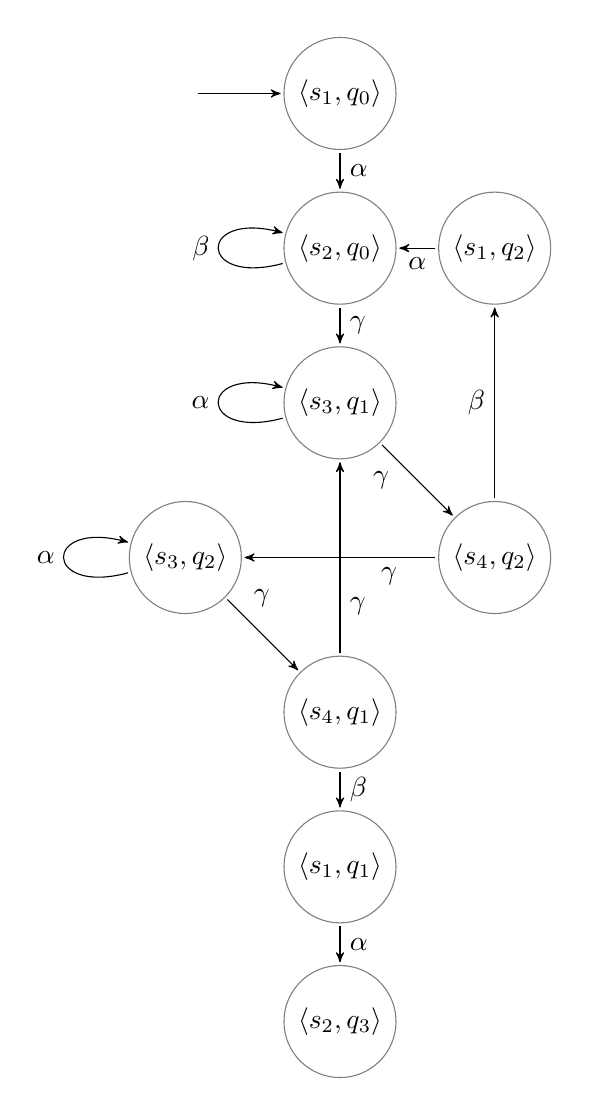
\begin{tikzpicture}[
                state/.style={
                    circle,
                    draw=black!50,
                },
                >= stealth',
                shorten >=1pt,
                shorten <=1pt,
            ]
            \matrix[column sep=1.5em, row sep=1.5em]{
                \node (start) {} ;
                    & \node [state] (s1q0) {\state{s_1}{q_0}} ;
                    & \\
                & \node [state] (s2q0) {\state{s_2}{q_0}} ;
                    & \node [state] (s1q2) {\state{s_1}{q_2}} ; \\
                & \node [state] (s3q1) {\state{s_3}{q_1}} ; & \\
                \node [state] (s3q2) {\state{s_3}{q_2}} ;
                    & & \node [state] (s4q2) {\state{s_4}{q_2}} ; \\
                & \node [state] (s4q1) {\state{s_4}{q_1}} ; & \\
                & \node [state] (s1q1) {\state{s_1}{q_1}} ; & \\
                & \node [state] (s2q3) {\state{s_2}{q_3}} ; & \\
            } ;

            \graph [ use existing nodes, ] {
                start ->
                s1q0 ->[edge label=$\alpha$]
                s2q0 ->[edge label=$\beta$, loop left]
                s2q0 ->[edge label=$\gamma$]
                s3q1 ->[edge label=$\alpha$, loop left]
                s3q1 ->[edge label=$\gamma$, near start, swap]
                s4q2 ->[edge label=$\gamma$, near start]
                s3q2 ->[edge label=$\alpha$, loop left]
                s3q2 ->[edge label=$\gamma$, near start]
                s4q1 ->[edge label=$\gamma$, near start, swap]
                s3q1 ;

                s4q1 ->[edge label=$\beta$]
                s1q1 ->[edge label=$\alpha$]
                s2q3 ;

                s4q2 ->[edge label=$\beta$]
                s1q2 ->[edge label=$\alpha$]
                s2q0 ;
            } ;
        \end{tikzpicture}
    \end{center}
    \caption{
        The synchronous product.
    }
    \label{fig:product}
\end{figure}

\section{(\#4.7) Checking equivalences of $\omega$-regular expressions}

\begin{enumerate}
        \enumalpha
    \item $(E_1 + E_2)F^\omega \equiv E_1 F^\omega + E_2 F^\omega$

        Take $\sigma$ in the LHS. If its prefix is recognized by $E_1$, then
        the left branch of the RHS will recognize it. Else, its prefix is
        recognized by $E_2$, in which case the right branch of the RHS will
        recognize it.

        Next take $\sigma$ in the RHS. Clearly, both
        $E_1 F^\omega \subset (E_1 + E_2) F^\omega$ and
        $E_2 F^\omega \subset (E_1 + E_2) F^\omega$.
        Since $\sigma \in E_1 F^\omega \union E_2 F^\omega$, we deduce that
        $\sigma \in (E_1 + E_2) F^\omega$.

    \item It is not the case that
        $E (F_1 + F_2)^\omega \equiv E_1 F^\omega + E_2 F^\omega$.

        To see this consider $E = \epsilon$, $F_1 = a$ and $F_2 = b$. The RHS
        recognizes either an infinite string of $a$ or an infinite string of
        $b$, yet the LHS recognizes an infinite string of possibly alternating
        $a$ and $b$.

    \item $E (F F^*)^\omega \equiv E F^\omega$

        The key is to see that $(F F^*)^\omega \equiv F^\omega$, since just
        prepending a equivalent regular expressions to equivalent
        $\omega$-regular expressions clearly gives equivalent $\omega$-regular
        expressions.

        Take $\sigma \in (F F^*)^\omega$. Clearly, for all $n \in \N$,
        $\sigma_n = F$. But then this is precisely what is understood by
        $\sigma \in F^\omega$. The reverse direction is even more obvious,
        since the count of ``$F$'' in the Kleene star can just be set to zero
        in each repetition in order to recognize any $\sigma \in F^\omega$.

    \item It is not the case that
        $(E^* F)^\omega \equiv E^* F^\omega$

        Consider $\sigma \in (E F)^\omega \subset (E^* F)^\omega$ the infinite
        string of alternations between $E$ and $F$. The machine identified with
        the expression in the RHS will enter a dead state once the second $E$
        is reached.
\end{enumerate}

% Note that to prove the above the above, we ``forgot'' that $E_*$ and $F_*$ were
% regular expressions and instead considered them as letters in an ``alphabet of
% regular expressions''. It's intuitively clear that 

\end{document}
